% Following colors are predefined: red, green, blue, cyan, magenta, yellow, black, gray, darkgray, lightgray, brown, lime, olive, orange, pink, purple, teal, violet and white.

\documentclass[tikz,border=1pt]{standalone}
\usetikzlibrary{shapes.misc, positioning}
\usetikzlibrary{external} 
\tikzsetexternalprefix{ffigurau} 
\tikzexternalize

\begin{document}
    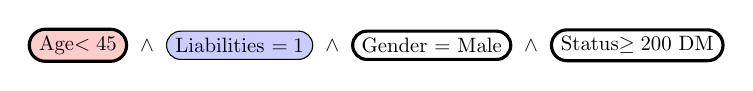
\begin{tikzpicture}[scale=1, every node/.style={scale=0.75}]
        \node (8) [fill=red!20, line width=0.4mm, draw, rounded rectangle] {Age$< 45$};
        \node (9) [right=of 8, xshift=-12.5mm] {$\wedge$};
        \node (10) [fill=blue!20, draw, right=of 9, xshift=-12.5mm, rounded rectangle] {Liabilities $=1$};
        \node (11) [right=of 10, xshift=-12.5mm] {$\wedge$};
        \node (12) [fill=white!20, line width=0.4mm, draw, right=of 11, xshift=-12.5mm, rounded rectangle] {Gender $=$ Male};
        \node (13) [right=of 12, xshift=-12.5mm] {$\wedge$};
        \node (14) [fill=white, line width=0.4mm,draw, right=of 13, xshift=-12.5mm, rounded rectangle] {Status$\geq 200$ DM};
    \end{tikzpicture}
% Age>=45, Gender=Female, Sta-tus<0 DM, Number liable=1
%   \begin{tikzpicture}
%     \draw (0,0) arc[radius=5pt,start angle= 90,end angle=270];
%     \draw (0,0) rectangle (40pt,-20pt);
%     \draw (40pt,0) arc[radius=5pt,start angle=90,end angle=-90];
%   \end{tikzpicture}
    % \node (2) [below=of 1, draw, rounded rectangle, rounded rectangle west arc=0pt] {rounded rectangle};
    % \node (3) [below=of 2, draw, rounded rectangle, rounded rectangle east arc=0pt] {rounded rectangle};
  
\end{document}